\documentclass[11pt,a4paper]{article}
\usepackage{cite,url,hyperref,graphicx, amsmath, bm}
\usepackage{alltt} 
\usepackage{listings}
\usepackage{algorithm2e} % need texlive-science which I'm having trouble with getting...
\lstset{
basicstyle=\small\ttfamily,
columns=flexible,
breaklines=true
}



\setlength{\textwidth}{6.5in}
\setlength{\oddsidemargin}{0in}
\setlength{\evensidemargin}{0in}
\setlength{\topmargin}{-0.5in}
\setlength{\textheight}{25cm}
%opening
\title{Error Analysis of PSMC'}
\author{Alex Lee Jackson}
\begin{document}

\maketitle

%\begin{abstract}
%blah
%
%\end{abstract}
\section{Miscellaneous}
For further inquiries, I can be contacted at \href{mailto:aj123@internode.on.net}{aj123@internode.on.net}, or DM'd on the \texttt{rstat} Slack.

GitHub: \url{https://github.com/alex-jackson1994/errorAnalysis}

\section{Objective}
Determine if there is a relationship between the level/type of chromosomal fragmentation, population model (predictor variables) and the error (response variable) in PSMC' (MSMC\cite{schiffels2014inferring} with two haplotypes). This will probably be analysed using mixed effects models.\\

\begin{algorithm}[H]
  \For{Each population model (3)}{
    \For{Each simulated genome (5)}{
      \For{Each model of fragmentation (2)}{
        \For{Each level of fragmentation (5)}{
          Run MSMC, record output.\
        }
      }
    }
  }
  Fit statistical model relating predictors to response.\\
  \caption{Outline of the simulation and MSMC analysis process}\label{overall}
\end{algorithm}

\section{Details}
PSMC' gives an estimate of how populations change over time, by analysing heterozygousity of sites across a genome (note: PSMC'/MSMC used interchangeably). However, real sequenced genomes will not always be nicely sorted into chromosomes. Often they will be assembled into smaller sections called contigs. We will simulate human genomes (as MSMC was originally written to analyse humans) under the following conditions:
\begin{itemize}
\item The length $L$ of the genome will be taken from a real human genome. For simplicity, \emph{only autosomes} will be considered.
\item Three different population models will be considered. In this document, take time $t$ as going from recent to ancient, i.e. $t=0$ is the more recent than $t=100$. These dynamics should be carefully considered, as we want them to fall into the time range where PSMC' can actually pick them up.
\begin{itemize}
\item Constant: $N_e(t)=N_0$.
\item Exponential decrease: $N_e(t)=N_0e^{kt}$ for some realistic $k<0$.
\item Bottleneck:
\begin{align*}
  N_e(t) = \begin{cases}
      N_0 & \text{if $0 < t < t_1$} \\
      N_0\exp\left\{\ln(\frac{N_1}{N_0}) \frac{t-t_1}{t_2-t_1} \right\} & \text{if $t_1 < t < t_2$}\\
      N_2 & \text{if $t_2 < t < \infty$}
    \end{cases}
\end{align*}

  A quick outline of this potential ``bottleneck'' model follows. Going from ancient to present, the population sits at constant level $N_2$. At time $t_2$, there's a bottleneck, and the population instantaneously drops to $N_1$. There's exponential growth until the population reaches $N_0$ at time $t_1$. From $t_1$ until present, the population remains constant at $N_0$. Of course, a different bottleneck model may be desired.
\end{itemize}
\end{itemize}



\subsection{Potential Whole Genome Simulators}
We want a simulator with the following properties.
\begin{itemize}
\item Able to simulate exponential growth.
\item Able to be converted to a format which can be taken by MSMC.
\item Able to simulate linkage disequilibrium (maybe... this may be introducing too much complexity).
\item Uses the coalescent model, not forward model (speed concerns?).
\item Can handle human genome sizes (in the range of 2.6 Gbp).
\item Can be converted to MSMC input format!
\end{itemize}
A number of simulators were considered.
\begin{itemize}
\item msHot-LITE (and ms, and msHot) (\url{https://github.com/lh3/foreign/tree/master/msHOT-lite}): This was used by Heng Li in his PSMC paper\cite{li2011inference}, and Schiffels, to simulate genomes. However, it has an upper size limit of roughly 10 Mbp.
\item GENOME (\url{http://csg.sph.umich.edu//liang/genome/}): This doesn't appear to do exponential growth.
\item GenomePop2 (\url{http://acraaj.webs.uvigo.es/GenomePop2.htm}): This can apparently output in ms-like format. Might go back to it later...
\item \textbf{MaCS} (\url{https://github.com/gchen98/macs}): Looking at this right now. It CAN handle the 2.6 Gbp sizes needed, as well as the other things I believe. Also, it's very fast.
\item \textbf{scrm} (\url{http://scrm.github.io/}): Recommended by Schiffels, but I haven't looked at it.
\end{itemize}

\subsubsection{MaCS}
For full detail, please refer to the MaCS README (\url{https://github.com/gchen98/macs/blob/master/README}), and the manual (\url{http://home.uchicago.edu/rhudson1/source/mksamples/msdir/msdoc.pdf}) for ms\cite{hudson2002generating}, from which MaCS is based upon. The MaCS README is fairly sparse, so I'd advise familiarising yourself with the relevant parts of the ms manual.

The MaCS README contains two examples of running MaCS. I'd advise taking the random seed, which is included in \texttt{stderr}, and storing it from each run. Alternatively, you could just specify the seed and store that each time. Reproducibility is important. From what I can gather, both \texttt{stderr} and \texttt{stdout} give useful things to use - simulated output goes to \texttt{stdout}, while tree statistics and other things go to \texttt{stderr}.

Further information can be found by running \texttt{./macs}. Note that:
\begin{itemize}
\item \texttt{<samplesize>} should always be 2, as we are simulating a diploid genome.
\item \texttt{<region in base pairs>} would be of the order of 2.6 Gbp. You should get this exactly from an empirical genome.
\end{itemize}
Switches of interest are: \texttt{-s} (sets seed from the Mersenne Twister algorithm), \texttt{-t} (sets mutation rate in units of mutations per site per $4N_0$ generations), \texttt{-r} (sets recombination rate in units of recombinations per site per $4N_0$ generations), \texttt{-T} (outputs in Newick format), \texttt{-eG} (sets growth rate, presumably in $N_0$ units), and \texttt{-eN} (sets population size in $N_0$ unis, sets growth rate to 0).

MaCS output should be able to be converted into the ms format via the included script \texttt{msformatter}. I've run this without errors, but haven't confirmed the ms format can then be converted to MSMC input format.

To convert from ms format to MSMC input format, use the script \texttt{ms2multihetsep.py}, included in the GitHub \url{https://github.com/stschiff/msmc-tools}. I haven't tried to use this yet.

\subsection{Simulation Parameters}
We will need the following parameters for the simulation.
\begin{itemize}
\item Genome size: obtaining this from an empirical human genome would be ideal. Remember, we are \emph{only considering autosomes}.
\item Mutation rate: Julien suggests $1.25\times 10^{-8}$ mutations per bp per generation is the current best estimate. 
\item Recombination rate: I don't know a good estimate.
\item Population models (this defines $N_0$ as well). We originally had Julien give us suggestions for times/effective sizes for a constant-bottleneck model. However, I suggest you guys all sit down and figure out exactly where you would like past demographic events to happen (as we want to make sure MSMC can pick them up).
\end{itemize}
Apart from the ``chromosome-level'' of fragmentation, fragmentation models will have to be discussed. This includes finding a relevant empirical contig distribution, and some mathematical model for chromosomal fragmentation (e.g. Poisson). Then you'll have to decide whether to do the fragmentation on the MaCS output, ms format, or the MSMC input.

\subsection{File Names And Data Frames}
This is up to you, but when we did the (unsuccessful) PSMC analysis we used the file names to store information about the simulation parameters. For example, say we had a MSMC output file corresponding to population demographic ``Constant'', simulated genome 2, fragmentation model ``Empirical'', and fragmentation level ``3''. Then the output file would be called something like \texttt{Constant\_2\_Empirical\_3.txt}. We could then use regular expressions in R to extract ``Constant'' etc. for storing in a data frame. Of course, there are lots of other ways it could be done!

See Table \ref{df} for an example of data frame we could use for storing results.
\begin{table}[h]
	\caption{Example data frame for storing analysis results. You might also want to add some summary statistics e.g. mean/variance of contig lengths.}
	\begin{center}
		\begin{tabular}{ccccc}
			\hline
			\textbf{Pop. Dem.} & \textbf{Sim. Number} & \textbf{Frag. Model} & \textbf{Frag. Level} & \textbf{Error} \\
                        \hline
                        Constant & 1 & Empirical & 1 & 2303 \\
                        Constant & 1 & Empirical & 2 & 4054 \\
                        \vdots & \vdots & \vdots & \vdots & \vdots \\
                        ExpDecr & 5 & Poisson & 5 & 1406 \\ \hline
		\end{tabular}
	\end{center} \label{df}
\end{table}


\subsection{Error Analysis}

\subsubsection{Definition Of Error}
We define the \emph{error rate} $\Delta (s_1,s_2)$ between two functions $s_1(t)$ and $s_2(t)$ as 
\begin{eqnarray}
\Delta (s_1,s_2) = \int_{t_R}^{t_A} |s_1(t)-s_2(t)| \,dt, \label{errorRate}
\end{eqnarray}
for sensible limits of integration $t_R$ (recent) and $t_A$ (ancient). Remember, treat recent time as time near 0, and ancient time as time towards $\infty$. The interpretation of this is the absolute value of the area between the two curves, in the interval $(t_R,t_A)$. Consult with Ben on choosing these values - a suggestion was the 95\% confidence interval for the time of coalescence between two haplotypes.

The limits of integration $T_R$ and $t_A$ should definitely ignore any data from the first time interval, and the last time interval. This is because Schiffels says \cite{schiffels2014inferring} ``the limits on the inference are given by the second and second-to-last boundaries, which correspond to the 2.5\% and 97.4\% quantile boundaries for the distribution of first coalescence times.''

Is error going to be evaluated on a log scale?

Are you going to compare fragmented results to the ``truth'' (simulation parameters of population which we specify), or to the ``best you can do'' (what MSMC recovers from the chromosomal level of fragmentation)?

\subsubsection{Calculating Errors}
Over the 2015/16 summer, the main script we used for calculating errors in PSMC was the following.
\begin{lstlisting}
~/Dropbox/MAGenomics_2015/PSMC_Scholarship/alexScripts/PSMC_Regression/StringExtraction_ErrorAnalysis.R
\end{lstlisting}
While this is optimised for the specific task we were doing, parts of it could be adapted for a MSMC analysis.

The main two functions of interest in the script are \texttt{eval\_popsize} and \texttt{absdifference}.

The function \texttt{eval\_popsize(pos, x, y)} takes a set of discrete points e.g. 
\begin{eqnarray*}
\{(t_1, N_{e}(t_1)), (t_2, N_{e}(t_2)), \cdots,(t_n, N_{e}(t_n))\}
\end{eqnarray*}
where \texttt{x} is a vector of $\{t_i\}$ and \texttt{y} is a vector of $\{N_e(t_i)\}$. Given a time point \texttt{pos}, the function will return the corresponding population size, if the $\{(t_i,N_e(t_i)) \}$ were connected by a step function. This allows us to construct the stepwise constant functions we see when MSMC graphs are plotted (see Figure \ref{pointsToStep}).

\begin{figure}
\centering
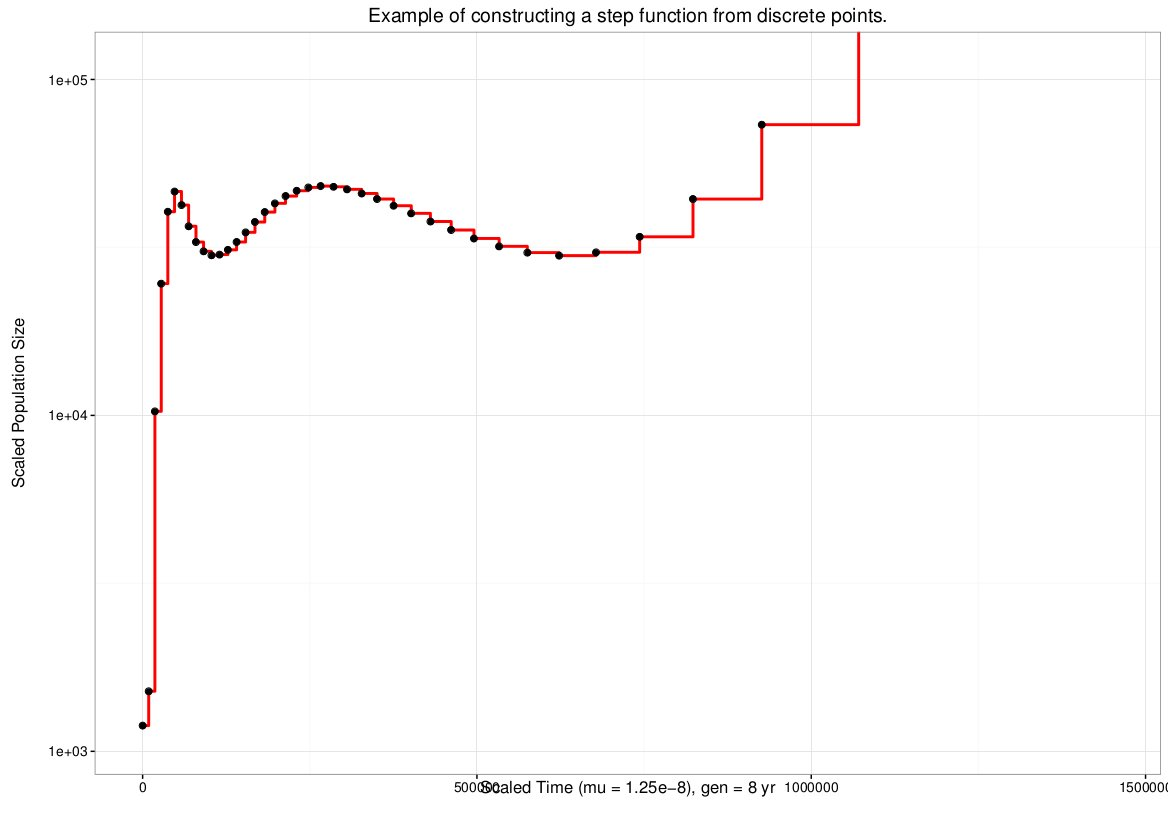
\includegraphics[width=1\textwidth]{pix/pointsToStep}
\caption{The function \texttt{eval\_popsize} allows us to construct a step function (red) from discrete points (black).} \label{pointsToStep}
\end{figure}

The function \texttt{absdifference(xpos,d1,d2,d3,d4)} returns the absolute difference between two MSMC stepwise constant functions $A$ and $B$, evaluated at point \texttt{xpos}. The other inputs to this function are \texttt{d1} and \texttt{d2} (vectors of $\{t_i\}$ and $\{N_e(t_i)\}$ respectively, for $A$), and \texttt{d3} and \texttt{d4} (vectors of $\{t_i\}$ and $\{N_e(t_i)\}$ respectively, for $B$). \texttt{absdifference} uses the \texttt{eval\_popsize} function.

One could then use R's integration function on \texttt{absdifference} to compute the integral that defines the error rate (Equation \ref{errorRate}).

Note that if you want to compare a ``true''  population model that involves curves (e.g. exponential growth) to MSMC output, the \texttt{absdifference} function may not be so useful. It might be better to write a new \texttt{absdifference} function which takes a MSMC stepwise constant function $A$ as one input, and a curve function $B$ as the other. However, this will be fine if comparing two MSMC curves (e.g. comparing the ``gold standard'' chromosomal fragmentation, with a much more fragmented genome).

\subsection{Running MSMC}
\subsubsection{Theory}
MSMC splits time from 0 (recent) to $\infty$ (ancient) into discrete unit time intervals. It then makes an estimate of population in each time interval. It then makes an estimate of the effective population in each interval (based on the heterozygousity of the genome).

The intervals are determined using the formula
\begin{eqnarray}
  t_i = \frac{-\ln (1-\frac{i}{n})}{{M\choose 2}} \label{timeInts}
\end{eqnarray}
for $i = 0, 1, \dots, n$. Here, $t_i$ is the time boundary of the particular interval, $n$ is the number of intervals (which you can define when running \texttt{msmc}), and $M$ is the number of haplotypes. As we will be looking at diploid individuals, the formula reduces to $t_i = -\ln (1-\frac{i}{n})$.

I am still a bit confused about exactly what units MSMC outputs its times in. Sorry!

The unit intervals can be combined. For example, if you were running MSMC using the command 
\begin{lstlisting}
msmc -p 30*1 [...]
\end{lstlisting}
then this would be instructing the program to use 30 unit intervals ($n = 30$). If you used 
\begin{lstlisting}
msmc -p 10*1+15*2 [...]
\end{lstlisting}
then the program would use 10 unit intervals followed by 15 double-unit intervals ($n = 40$) (this also happens to be the default pattern). The left of \texttt{10*1+15*2} corresponds to recent time and the right corresponds to ancient time and the right corresponds to ancient time.

In the MSMC and PSMC papers, I have not found any justification for the use of particular combinations of time intervals.

I have found that if you scale MSMC time output such as in \texttt{plotMSMC\_PSMC.R}, you will \emph{not} get the same times as you do when you rescale the numbers you take from Equation \ref{timeInts}. To get the same times, you need to rescale by MSMC's estimate of mutation rate (which you should be able to find as \texttt{mutationRate} in the \texttt{log} file outputted by MSMC).

If you are interested, the recombination rate estimate \texttt{recombinationRate} can also be found in the \texttt{log} file.

\subsubsection{Using Real Data}
See attached example \texttt{runMSMC.txt}, which uses the Tasmanian Devil data. Julien should also be able to help with this. This will give a quick run-through of what the different commands are doing.

\begin{lstlisting}
awk '{print $1, 0, $2, $1, "0", "+"}' [...]
\end{lstlisting}
MSMC requires individual text input files per chromosome or contig. In this case, we look at the Devil \texttt{fasta} reference file to find the largest contigs to use. In this particular case, we only decided to use the contigs that were larger than 5 Mbp.

\begin{lstlisting}
module load python/4.8.0/3.4.1 gnu/4.9.2 zlib/testing samtools/1.2 bcftools/1.2 msmc/20150413 htslib/1.2.1 parallel
\end{lstlisting}
Load the relevant modules.

\begin{lstlisting}
parallel -j7 --nice 19 "samtools mpileup -EA -Q 20 -C 50 -u -r {} -f /localscratch/Refs/Sarcophilus_harrisii/Devil7_0_Raw [...]
\end{lstlisting}
You and Julien probably have a better idea of this than me. This creates the MSMC input files. For a different genome, obviously the names would have to be different. A \texttt{bam} genome and a \texttt{fasta} reference are required.

The next part is a copy from one of my files, 
\begin{lstlisting}
/localscratch/jsoubrier/Bison_Genomes/CowRef/AlexPSMCMSMC_Comparison/labBook
\end{lstlisting}
and should highlight relevant MSMC commands. Further information can be found on the GitHub guide (\url{https://github.com/stschiff/msmc/blob/master/guide.md}) or by running \texttt{msmc} on its own.
\begin{lstlisting}
msmc -t 50 -p 40*1 -i 20 -o EuropeanBison.Cow_UMD3_1.realigned_AllAutosomes_MSMCOutput EuropeanBison.Cow_UMD3_1.realigned_chr1_MSMCInput.txt EuropeanBison.Cow_UMD3_1.realigned_chr2_MSMCInput.txt [...] | at now
\end{lstlisting}
The switches of interest are: \texttt{-t} (sets number of threads to run on), \texttt{-p} (set how MSMC chooses and combines its time intervals), \texttt{-i} (number of iterations... I don't now a good way to choose this, I've been using 20), and \texttt{-o} (set the name of the output file). The \texttt{--fixedRecombination} flag should be left out for running on two haplotypes (our situation), according to the guide.

Following the name of the output file are the MSMC input files (there were 29 in this case). This can make the commands long and messy. Finally, the \texttt{| at now} allowed me to leave this running on the server and then log off.

\subsubsection{Using Simulated Data}
I am not sure how to do this, but presumable it would go something like this:
\begin{enumerate}
\item Run MaCS (or similar) with the \texttt{-T} flag to output in the appropriate format.
\item Convert this to ms output format with the \texttt{msformatter} script which comes with MaCS. See \ref{sec:ms} for more detail on this file format.
\item Convert this to MSMC input format with \texttt{ms2multihetsep.py} included with Schiffels' MSMC tools. 
\item (Fragment somewhere in above.)
\item Run MSMC as above.
\end{enumerate}

\subsection{Visualising MSMC}
See the attached example file \texttt{plotMSMC\_PSMC.R} for an annotated R file which runs through plotting MSMC (and PSMC). Just remove the parts relevant to PSMC if you only care about MSMC.


\section{Other Suggestions}
\subsection{Reduction In Complexity}
Julien suggested that we could do some trials to see if we recover the same dynamics with say 5 chromosomes, instead of the full 23. This would significantly decrease the run-time of the whole progress. However, fragmenting 5 chromosomes may be quite different to fragmenting 23 chromosomes.

\subsection{Looking At Bias}
We are more looking at the variability in the MSMC estimate. To look at bias, this would probably require a different definition of error rate.

\subsection{Hybridisation}
TBD.

\section{PSMC}
\subsection{Background}
The Pairwise Sequentially Markovian Coalescent (PSMC) model \cite{li2011inference} is a method for estimating past population dynamics based on the  genome of a single individual. PSMC uses the heterozygousity of the genome to estimate where recombination events have occurred in the genome. These estimates are found using a Hidden Markov Model (for an introduction to HMMs, see the paper by Rabiner \cite{rabiner1989tutorial}). A genome is split into many consecutive, non-overlapping 100 bp ``bins''. The observations are whether each of the bins contains a heterozygous pair (``1''), is homozygous (``0''), or data is missing (``.''). The state space is the set of non-overlapping time intervals from the present back in time. The hidden state is the time interval into which the TMRCA for each bin falls. This allows PSMC to then construct a population estimate over a period of time. 

For further detail, see the paper by Li \cite{li2011inference} (the Methods section in particular gives a starting point) as well as the supplementary information for detail, and the package's README at \url{https://github.com/lh3/psmc}.
\subsection{PSMC vs MSMC}
The key differences between PSMC and MSMC are as follows:
\begin{itemize}
\item PSMC can only be run on a diploid genome, while MSMC can be run on more than two haplotypes.
\item PSMC partitions the genome into 100 bp ``bins''. Each bin is then assigned either heterozygous or homozygous (or missing). MSMC does not need this, as its software is more efficient.
\item MSMC allows for a ``null recombination'' event, which if I've interpreted Ben correctly, is a recombination which immediately coalesces back into the same branch... or something. PSMC ignores this.
\item PSMC and MSMC have different ways of splitting up time from 0 to infinity. MSMC's formula is 
\begin{align*}
t_i = \frac{-\ln (1-\frac{i}{n})}{{M\choose 2}}
\end{align*}
as mentioned above. PSMC's formula is 
\begin{align*}
t_i = 0.1\exp\left\{ \frac{i}{n}\ln(1+10T_{\text{max}}) \right\},
\end{align*}
for $i = 0, 1, \dots, n$. The parameter $T_{\text{max}}$ is the maximum TMRCA, which can be specified when running \texttt{psmc} using the \texttt{-t} switch (in units of $2N_0$, the default is 15). PSMC output is scaled to $2N_0$ - unfortunately, I'm not sure what the units are in the above equation.

For an equivalent amount of time intervals, PSMC's time intervals reach more into recent time than MSMC's do. Nigel thinks this is because recent estimates are rubbish, so MSMC effectively ignores them.
\item Apparently, MSMC estimates recombination rate better than PSMC.
\item There are probably also some subtle mathematical differences which Ben and Jono will have to go over when they analyse the equations.
\item The underlying model of PSMC is the SMC model\cite{mcvean2005approximating}, while the underlying model of PSMC' is the SMC' model\cite{marjoram2006fast}.
\end{itemize}

\subsection{Running PSMC On Real Data}
Similarly to MSMC, we start with a \texttt{fasta} and a \texttt{bam}. We use samtools and related software to produce a \texttt{fastq} output file. This uses the kangaroo as an example.
\begin{lstlisting}
samtools mpileup -EA -Q20 -C50 -u -f Macropus_eugenii.Meug_1.0.dna_rm.toplevel.fasta Kangaroo.Meug_1_0.realigned.bam | bcftools call -c | vcfutils.pl vcf2fq | gzip > mpileupedKangaroo.fq.gz
\end{lstlisting}
We then convert the \texttt{fastq} to the PSMC input format, \texttt{psmcfa} (see Appendix \ref{sec:psmcfa} for detail on this format). The \texttt{fq2psmcfa} script is included with PSMC's utils.
\begin{lstlisting}
fq2psmcfa redKangaroo.fq.gz > redKangaroo.psmcfa
\end{lstlisting}
We then run PSMC (here using the bison example). Switches used here are \texttt{-p} (specifies number of time intervals and how they're combined, like in MSMC) and \texttt{-N}, the number of iterations.
\begin{lstlisting}
/localscratch/Programs/psmc/psmc -p 40*1 -N 20 EuropeanBisonFullGenome29Autosomes.psmcfa > EuropeanBison29Autosomes_Int40*1_Iter20.psmc | at now &
\end{lstlisting}
We still need to extract the data from PSMC if we wish to plot it, or analyse the error. Shaun wrote a script, \texttt{removeDataFromPSMC.sh}, which does this for us (in the \texttt{scripts} folder). It is run as follows. You will still need the \texttt{psmc} file to obtain $\theta_0$, which is required for plotting PSMC output (see the example \texttt{plotMSMC\_PSMC.R}).
\begin{lstlisting}
./removeDataFromPSMC.sh PSMC/EuropeanBison29Autosomes_Int40*1_Iter20.psmc > PSMC/EuropeanBison29Autosomes_Int40*1_Iter20.psmcData
\end{lstlisting}

\subsection{Running PSMC On Simulated Data}
If you simulate your genome in the \texttt{ms} format, Heng Li has written the script \texttt{ms2psmcfa.pl} to convert to the \texttt{psmcfa} format. This is included in the PSMC utils.

If you use \texttt{msHOT-lite} (probably not recommended) to run your simulation, you need to use the \texttt{-l} switch to ensure the format is correct for PSMC. If you use MaCS or something similar, I'm not sure of what you'll have to do. MaCS' \texttt{msformatter} script might be adequate.

\begin{lstlisting}
msHOT-lite 2 1 -t 60000 -r 10000 1000000 -eN 1 2 -eN 2 4 -l > output.ms
perl ms2psmcfa.pl input.ms > output.psmcfa
\end{lstlisting}

\subsection{Goodness of Fit, And Correcting for False Negatives}
Li \cite{li2011inference} has devised methods for checking goodness of fit, but I don't understand how to test this. In Section 2.2 of the Supplementary Information, he gives detail. There does not appear to be a script for extracting the statistics though.

In the S.I., Li says that you can check $C_\sigma\pi_k$ for overfitting. If it's small (e.g. less than 20), you shouldn't trust the estimates of $\lambda_k$. I'm not sure how to get this value though.

In Appendix II of the PSMC README file, Li talks about correcting for false negatives in the case of low coverage (for example, the kangaroo only had 55\% coverage). I'm not sure how to estimate this.

\subsection{Scripts Which Might Be Useful}
\begin{table}[h]
\begin{tabular}{p{6.5cm}p{8.5cm}}
  \hline
  \textbf{Name} & \textbf{Description} \\ 
  \hline
  \texttt{combinePsmcfa.sh} & Combines all contigs in a \verb|.psmcfa| file to create one giant contig! \\ \hline
  \parbox[t]{5cm}{\texttt{findNLargestContigs.py} *} & From a \texttt{psmcfa} file, creates a new \texttt{psmcfa}, only containing data from the \texttt{N} largest contigs (\texttt{N} user-specified) Uses \texttt{python3}.\\ \hline
  \texttt{growthDataSlidingWindowError.R} & Does a sliding window-style error analysis. \\ \hline
  \parbox[t]{5cm}{\texttt{removeDataFromPSMC.sh} *} & Extracts time, population estimates etc. from \texttt{psmc} files, in a tab-delimited format.\\ \hline
  \texttt{removeRandomContigs.py} & Removes contigs randomly from a \verb|.psmcfa| file.\\ \hline  
  \texttt{removeRandomPartsFromPsmcfa.py} & Removes lines randomly from a \verb|.psmcfa| file.\\ \hline  
  \parbox[t]{5cm}{\texttt{StringExtraction\_ErrorAnalysis.R}} & Extracts information about the specific simulation with regular expressions. Runs error analysis and creates data frame. Well commented, but very messy though.\\ \hline
\end{tabular}
\end{table}


\appendix
\section{File Types}
Thanks to Shaun Barker, who wrote this over the summer.
\subsection{MS (.ms)}\label{sec:ms}
	MS (.ms) files are simulated output from msHOT-lite (as well as MS, SCRM and other MS derivatives). It was written by Heng Li (who also created the PSMC software and others software used in bioinformatics). It contains a list of genome fragments (e.g. chromosomes/contigs/scaffolds), and in each of those fragments it lists the positions of heterozygous pairs as well as the type. The file begins with the call that created the file then each chromosome generated is listed. Each chromosome is stored between a \verb|@begin| and \verb|@end| statement. An example of an MS file can be seen in Figure \ref{msFile}.
	\begin{figure}[h]
		\begin{lstlisting}
		./msHOT-lite 2 1 -t 30000 -r 6000 300000 -eN 0.01 0.1 -eN 0.06 1 -eN 0.2 0.5 -eN 1 1 -eN 2 2 -l 
		//
		@begin 11765
		300000
		37295	10
		81727	01
		104834	01
		131283	01
		191522	10
		298343	01
		@end
		\end{lstlisting}
		\caption{An example of a MS file.}
		\label{msFile}
	\end{figure}
For further detail, see the ms paper by Hudson REF and the msHOT-lite repository at \url{}.

\subsection{PSMC Input Files (.psmcfa)}\label{sec:psmcfa}
PSMC input files (.psmcfa) are plain text files (see Figure \ref{psmcfa}) generated by many of the utilities provided alongside PSMC. They are the only input files required by PSMC. The .psmcfa files contain a list of chromosomes/contigs/etc. and 60 character wide lines that denote where heterozygous pairs occur. Each character in the lines represent the bin  $[100i,100i+100)$ along the sequence, for each $i$ sequential non-overlapping 100bp bin along length of the sequence. The character is K if there is a heterozygous pair in that bin of the sequence, T if the bin is completely made of homozygous pairs, and N if the data is too low quality or missing.
	\begin{figure}[h]
		\begin{lstlisting}
		>thisIsTheFirstSequenceName
		TKTKTKKTKTKTKTKTKKTKTKTKKKKKKKKTTTKKTKTKTKTKTKTKKTKTTKTKTKTK
		KKKKTKKKKTKKKKKKKKTTTTTTTTTKKTKTKKKKKKKKKKKKKKKKKKKKKKKKKKTT
		TTTTTTTTTTTTTKKKKKKKKKKTKKKKTKKKKKKKKKKKKKKKKKKKTTKKKKKKKKKK
		TKKKTKTKKTKTKKTKTTTKTKTKTKTKTTKKTTKTKTKKKTKTKTKTKKTTTKTKTTKK
		>thisIsTheSecondSequenceName
		KKKKKKKKKKKKKKKKKKKKKKKKKKKKKKKKKKKKKKKKKKKKKKKKKKKKKKKKKKKK
		KKKKKKKKKKKKKKKKKKKKKKKKKKKKKKKKKKKKKKKKKKKKKKKKKKKKKKKKKKKK
		TTTTTTTTTTTTTTTTTTTTTTTTTTTTTTTTTTTTTTKTTTTTTTTTTTTTTTTTTTTT
		TTTTTTTTTTTKTTTTTTTTTTTTTTTTTKTTTTTTTTTTTTTTTTTTTTTTTTTKTTTT
		\end{lstlisting}
		\caption{An example of a .psmcfa file.}\label{psmcfa}
	\end{figure}
	
\subsection{PSMC Output Files (.psmc)}
The .psmc output files are plain text files outputted by PSMC. They contain details on the iterations performed by the program and the values. They all have a header describing the file itself (see Figure \ref{psmcHeader}) and this should be read to attempt to understand the output. The final table in the .psmc file is the ``final'' result after 20 iterations of expectation-maximisation, and can be extracted with the \verb|removeDataFromPSMC.sh| script.

Note: According to a comment by Heng Li at \url{https://hengli.uservoice.com/forums/152783-general/suggestions/6787405-shouldn-t-the-pi-k-column-in-the-psmc-output-be-be}, the \verb|\pi_k| column is not actually \verb|\pi_k|. It may be \verb|\sigma_k| instead.

	\begin{figure}[h]
		\begin{lstlisting}
                  CC
                  CC	Brief Description of the file format:
                  CC	  CC  comments
                  CC	  MM  useful-messages
                  CC	  RD  round-of-iterations
                  CC	  LL  \log[P(sequence)]
                  CC	  QD  Q-before-opt Q-after-opt
                  CC	  TR  \theta_0 \rho_0
                  CC	  RS  k t_k \lambda_k \pi_k \sum_{l\not=k}A_{kl} A_{kk}
                  CC	  DC  begin end best-k t_k+\Delta_k max-prob
		\end{lstlisting}
		\caption{The header description of a .psmc file.}\label{psmcHeader}
	\end{figure}

The output files generated by PSMC are a (roughly) tab delimited text format, where the first two characters on each line defines what values are on the line. The output files always contain a header which gives some information on the format, and then parameter estimates for each iteration of the Baum-Welch algorithm used in PSMC. The last table contains the estimates from the final iteration, this is the data we used for our analysis. The last table can be extracted as a tab delimited table using the script \verb|removeDataFromPSMC.sh|. This script takes a \verb|.psmc| output file as its input and then outputs the final table in the file as a tab delimited text file.

PSMC gives scaled output \cite{li2011inference}. The time $t_k$ is in terms of 2$N_0$ generations. The population given is in terms of $\lambda_kN_0$, which is the proportion relative to $N_0$. $N_0$ is defined as ``effective population size'', but what that means specifically is unclear. $N_0$ can be obtained by the formula $N_0=\theta/(4\mu s)$.

\bibliographystyle{plain}
\bibliography{../references/references}{}


\end{document}
